% PA3 report skeleton. Replace the style line with the course NeurIPS template from PA0.
% Figures/tables are generated by task*/analyze.py into ../results/...; numbers are filled in after the GPU runs.
\documentclass{article}
\usepackage[final]{neurips_2024}   % <-- swap for the PA0 course style file
\usepackage{graphicx,booktabs,amsmath,amssymb,hyperref,xcolor}
\graphicspath{{../results/}}
\newcommand{\todo}[1]{\textcolor{red}{[TODO: #1]}}

\title{Adaptation, Grounding, and Test-Time Compute in Small Language and Vision-Language Models}
\author{\todo{name} \\ \todo{roll number}}

\begin{document}
\maketitle

\begin{abstract}
\todo{3--4 sentences per task: setup, main quantitative finding, main caveat.}
Code: \url{https://github.com/adilawan1/ATML-PA3}.
\end{abstract}

\section{Introduction}
\todo{Motivation: adaptation vs.\ retention; visual evidence vs.\ language priors; when extra inference compute helps.}

\section{Experimental Setup}
All runs use seed 6304 and a single GPU type (\todo{GPU, e.g.\ NVIDIA L4 24\,GB}); every reported number is regenerated by the scripts in the repository. Full hyperparameters and implementation decisions are in Appendix~\ref{app:details}.

\paragraph{Task 1: fine-tuning and retention.} We fine-tune Qwen3-0.6B~\cite{yang2025qwen3} in non-thinking mode on the first 40{,}000 eligible MetaMathQA~\cite{yu2024metamath} examples in source order (2 of the first 40{,}002 rows exceed 2{,}048 tokens; none match a GSM8K test question after normalization). The selection contains 9.91M tokens, of which 7.10M are supervised response tokens. Each run makes one pass: 1{,}250 AdamW updates at effective batch 32, linear warmup over 38 updates and cosine decay, gradient clipping at 1.0, and FP16 autocast with dynamic loss scaling. We compare five variants: Full FT (LR $2\times10^{-5}$), Full FT with L2-SP~\cite{li2018l2sp} ($\lambda=10^{-3}$), LoRA~\cite{hu2022lora} with $r=4$ and $r=16$ ($\alpha=2r$, LR $2\times10^{-4}$, all seven attention and MLP projections), and OPLoRA~\cite{xiong2025oplora} with $r=16$ and $k=128$ protected singular directions. LoRA-16 and OPLoRA-16 start from identical adapter factors. Seven conditions are evaluated: the baseline, Full FT at its midpoint (625 updates), and the five final models. Specialization is measured on GSM8K~\cite{cobbe2021gsm8k} (\texttt{gsm8k\_cot}, zero-shot, greedy, 1{,}024 new tokens, non-thinking chat template); retention on HellaSwag~\cite{zellers2019hellaswag}, BoolQ~\cite{clark2019boolq} and ARC-Easy~\cite{clark2018arc} by likelihood scoring, all with lm-evaluation-harness 0.4.13~\cite{evalharness} on complete splits. Weight-space diagnostics on \texttt{down\_proj} at layers 0, 13 and 27 report the fraction $\rho_k$ of the update in the protected output subspace, the relative magnitude $\eta=\|\Delta W\|_F/\|W_0\|_F$, and the activation response ratio $R(z)$ on a fixed set of 32 math (GSM8K) and 32 non-math (HellaSwag) probes. A qualitative set of 24 prompts~\cite{betley2025emergent} is answered greedily by every condition.

\paragraph{Task 2: a small VLM and visual grounding.} Frozen SigLIP-B/16~\cite{zhai2023siglip} features (196 post-LayerNorm tokens of dimension 768, cached in FP16) pass through a two-layer GELU MLP connector ($768\to1024\to1024$) and replace \texttt{<|image\_pad|>} embeddings inside Qwen3-0.6B's chat format. The connector output is multiplied by a fixed scale, set at initialization so that visual tokens match the mean norm of text-token embeddings on training data. Training follows three stages at effective batch 16: (1) caption alignment on 18{,}000 COCO~\cite{lin2014coco} captions (6{,}000 images, 2{,}250 updates, connector only); (2) visual instruction tuning on generated presence and counting questions plus captions (1{,}500 updates); (3) natural VQA on VQAv2~\cite{goyal2017vqa2} complementary pairs mixed with the earlier data (750 updates). Stages 2--3 add LoRA ($r=16$) to the attention projections; the LLM and vision encoder stay frozen. Grounding is tested on 64 generated pairs (32 presence, 32 counting) and 96 VQAv2 complementary pairs (36 yes/no, 24 number, 36 other) whose two questions share text but differ in image and answer. Each question is answered under four image conditions: correct image, the pair partner's image, a mismatched image, and no image. We report exact match (generated suites) or VQA soft accuracy, pair accuracy, partner-follow rate and reference-answer NLL, with 95\% CIs from 4{,}000 pair-level bootstrap resamples.

\paragraph{Task 3: test-time compute.} We analyze the supplied pools of 32 sampled rollouts per question for MATH~\cite{hendrycks2021math} (Qwen2.5) and MathVista~\cite{lu2024mathvista} (Qwen2.5-VL), 1{,}000 questions each, split once into 200 development and 800 held-out questions. Answers are grouped without gold labels (math-verify~\cite{mathverify} equivalence for MATH, MathVista's official normalization for MathVista). For budgets $N\in\{1,2,4,8,16,32\}$ and 10 seeded rollout orders we compare first-answer, self-consistency~\cite{wang2023selfconsistency}, maximum log-probability, maximum self-certainty~\cite{kang2025selfcertainty}, and rank-weighted consensus (RWC); on MathVista also visual-attention, VisConf~\cite{usman2025visconf} and token-wise fused scores. All scores and calibrations use only the revealed candidates. Adaptive stopping checks agreement after 4, 8 and 16 rollouts, with thresholds tuned on the development split and frozen for the held-out split. A live run on 50 held-out MATH questions with Qwen2.5-3B-Instruct gives each strategy the same 3{,}072-token output allowance: one long response, three parallel 1{,}024-token responses with self-consistency, or one response followed by a 2{,}048-token critique and revision~\cite{madaan2023selfrefine}. Paired question-level bootstrap (1{,}000 resamples) gives CIs throughout.

\section{Results and Analysis}
\subsection{Task 1: Fine-tuning, adaptation and retention}
\begin{table}[t]\centering\small
\begin{tabular}{lrrrrrrrr}
\toprule
condition & GSM8K (flex EM) & Δ GSM8K (flex EM) (pp) & HellaSwag (acc_norm) & Δ HellaSwag (acc_norm) (pp) & BoolQ (acc) & Δ BoolQ (acc) (pp) & ARC-Easy (acc_norm) & Δ ARC-Easy (acc_norm) (pp) \\
\midrule
Baseline & 43.1 & 0.0 & 47.3 & 0.0 & 64.3 & 0.0 & 56.1 & 0.0 \\
Full FT (mid) & 57.1 & 14.0 & 45.7 & -1.6 & 61.0 & -3.3 & 62.9 & 6.9 \\
Full FT & 64.4 & 21.4 & 46.1 & -1.2 & 58.8 & -5.5 & 63.8 & 7.7 \\
Full FT + L2-SP & 65.2 & 22.1 & 46.5 & -0.9 & 67.4 & 3.1 & 63.6 & 7.6 \\
LoRA-4 & 59.7 & 16.6 & 47.2 & -0.1 & 69.3 & 5.0 & 63.0 & 6.9 \\
LoRA-16 & 62.3 & 19.3 & 47.2 & -0.1 & 72.1 & 7.7 & 63.0 & 6.9 \\
OPLoRA-16 & 62.2 & 19.1 & 46.9 & -0.4 & 72.4 & 8.0 & 62.9 & 6.9 \\
\bottomrule
\end{tabular}

\caption{Primary scores (\%) and change from the shared baseline (pp) for the seven evaluation conditions.}\label{tab:t1}
\end{table}
\begin{figure}[t]\centering
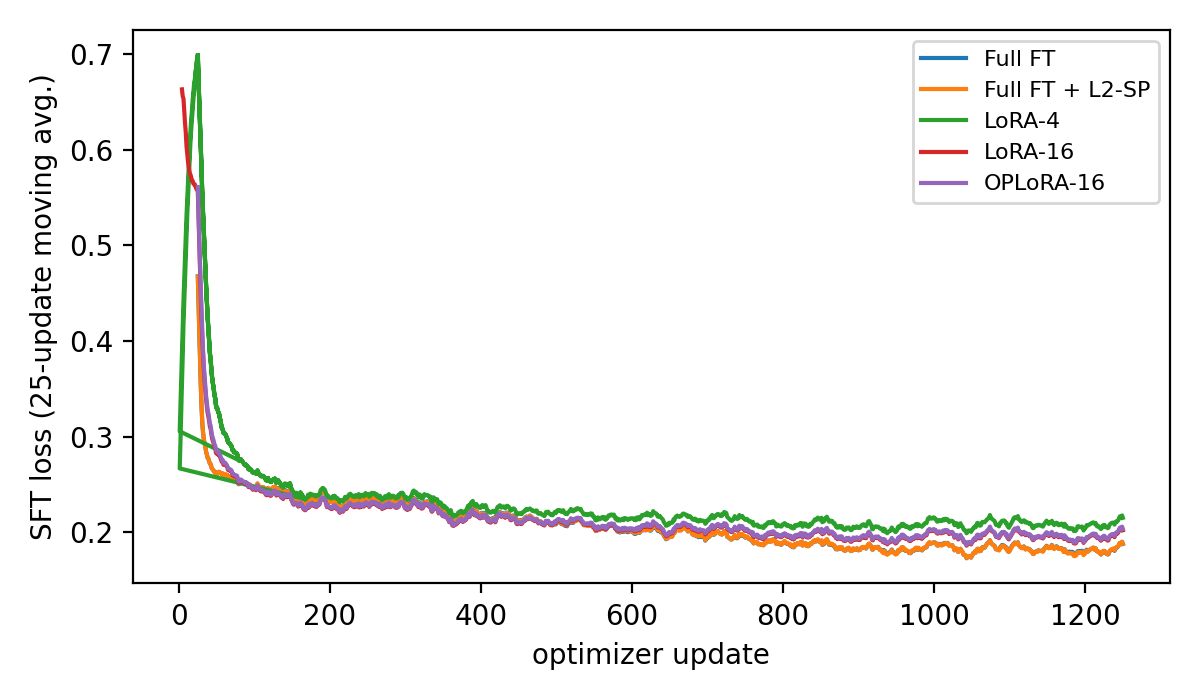
\includegraphics[width=.48\linewidth]{task1/report/sft_loss.png}\hfill
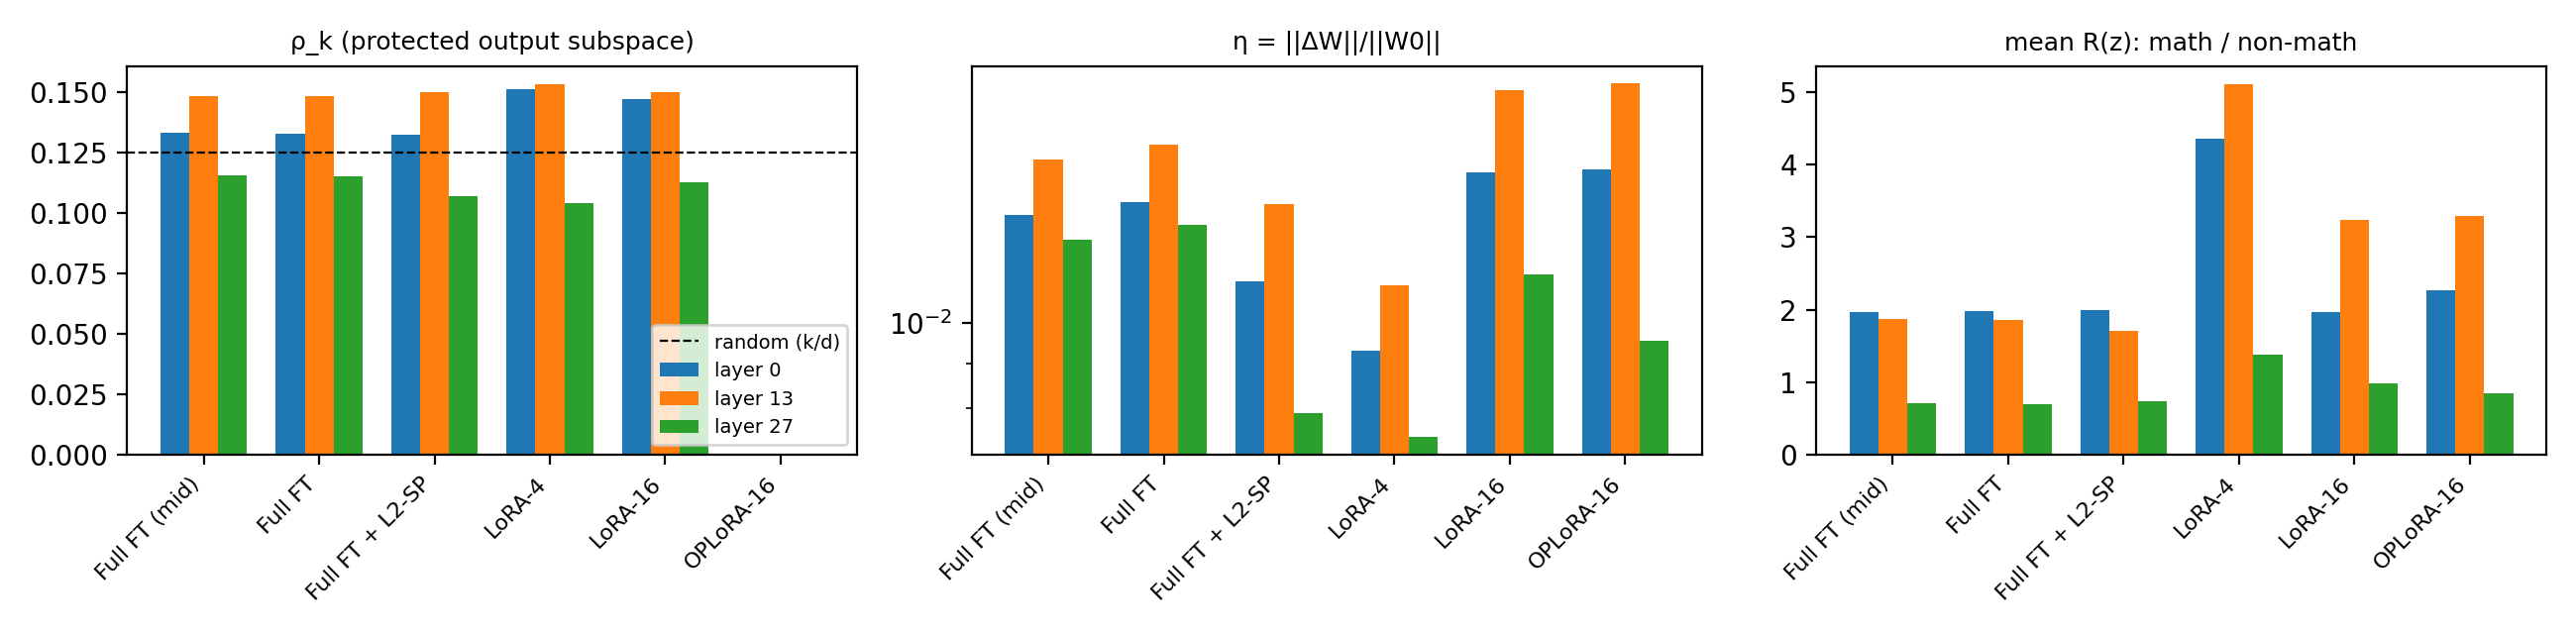
\includegraphics[width=.48\linewidth]{task1/report/diagnostics.png}
\caption{Left: SFT loss for the five runs. Right: $\rho_k$, $\eta$, and math/non-math $R(z)$ for \texttt{down\_proj} (layers 0/13/27).}\label{fig:t1}
\end{figure}
\todo{RQ1 specialization vs.\ retention (incl.\ Full FT midpoint); RQ2 restrictions (rank, L2-SP, OPLoRA); RQ3 geometry vs.\ behaviour (and what diagnostics cannot establish); RQ4 cost (resources table); RQ5 qualitative (42-response annotation, aligned excerpts, selection rule).}

\subsection{Task 2: Visual grounding}
\begin{figure}[t]\centering
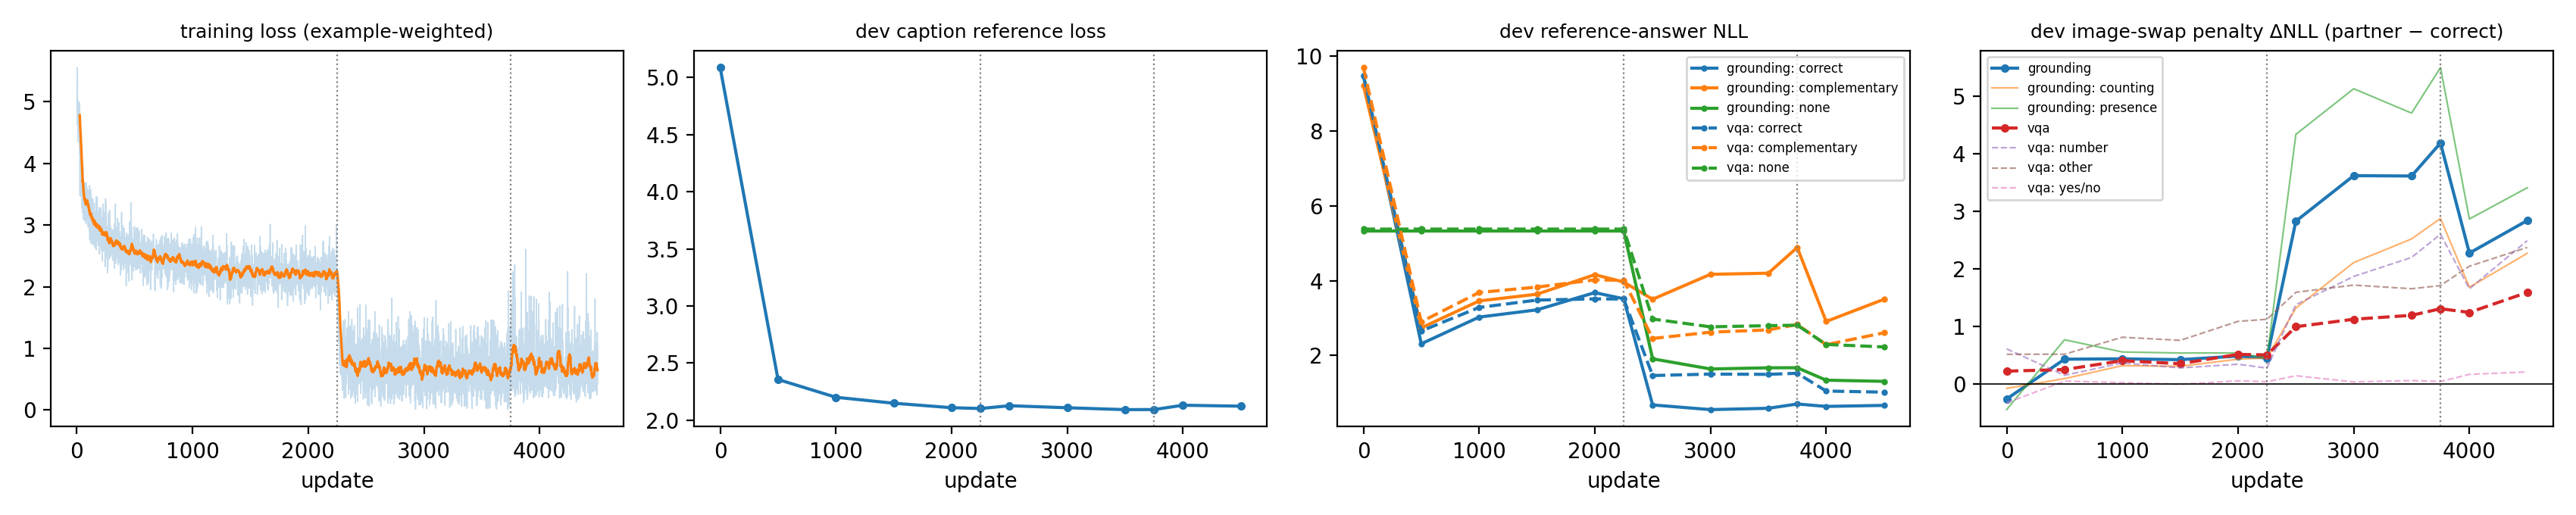
\includegraphics[width=\linewidth]{task2/vis196/report/curves.png}
\caption{Training loss and development metrics; dotted lines mark stage boundaries.}\label{fig:t2}
\end{figure}
\begin{table}[t]\centering\small
\begin{tabular}{llllrrlrr}
\toprule
suite & condition & accuracy % [95% CI] & pair acc % & identical % & empty % & ref NLL & partner-follow % & ms/answer \\
\midrule
Annotation-derived grounding & correct & 68.8 [59.4, 78.1] & 54.7 [42.2, 67.2] & 21.9 & 0.0 & 0.8 [0.6, 1.1] & 14.1 & 23.1 \\
Annotation-derived grounding & complementary & 14.1 [8.6, 20.3] & 1.6 [0.0, 4.7] & 21.9 & 0.0 & 3.4 [3.1, 3.8] & 68.8 & 18.6 \\
Annotation-derived grounding & mismatched & 32.8 [25.8, 39.1] & 3.1 [0.0, 7.8] & 75.0 & 0.0 & 2.1 [1.9, 2.4] & 31.2 & 18.8 \\
Annotation-derived grounding & none & 40.6 [35.2, 45.3] & 0.0 [0.0, 0.0] & 100.0 & 0.0 & 1.2 [1.1, 1.4] & 40.6 & 17.9 \\
Natural VQAv2 & correct & 54.5 [47.6, 61.5] & 29.2 [20.8, 38.5] & 43.8 & 0.0 & 1.4 [1.1, 1.7] & 26.8 & 26.2 \\
Natural VQAv2 & complementary & 26.8 [21.1, 32.9] & 4.2 [1.0, 8.3] & 43.8 & 0.0 & 2.8 [2.4, 3.3] & 54.5 & 25.9 \\
Natural VQAv2 & mismatched & 29.2 [23.6, 34.8] & 2.1 [0.0, 5.2] & 62.5 & 0.0 & 2.6 [2.2, 3.1] & 31.0 & 23.1 \\
Natural VQAv2 & none & 30.0 [24.8, 35.3] & 0.0 [0.0, 0.0] & 100.0 & 0.0 & 2.4 [2.1, 2.9] & 30.0 & 21.7 \\
\bottomrule
\end{tabular}

\caption{Final-test results under four image conditions (95\% pair-bootstrap CIs).}\label{tab:t2}
\end{table}
\todo{RQ1 curriculum; RQ2 grounding: generated vs.\ natural questions, partner-follow; RQ3 NLL vs.\ generation vs.\ pair metrics; RQ4 capabilities and cost.}

\subsection{Task 3: Test-time compute}
\begin{figure}[t]\centering
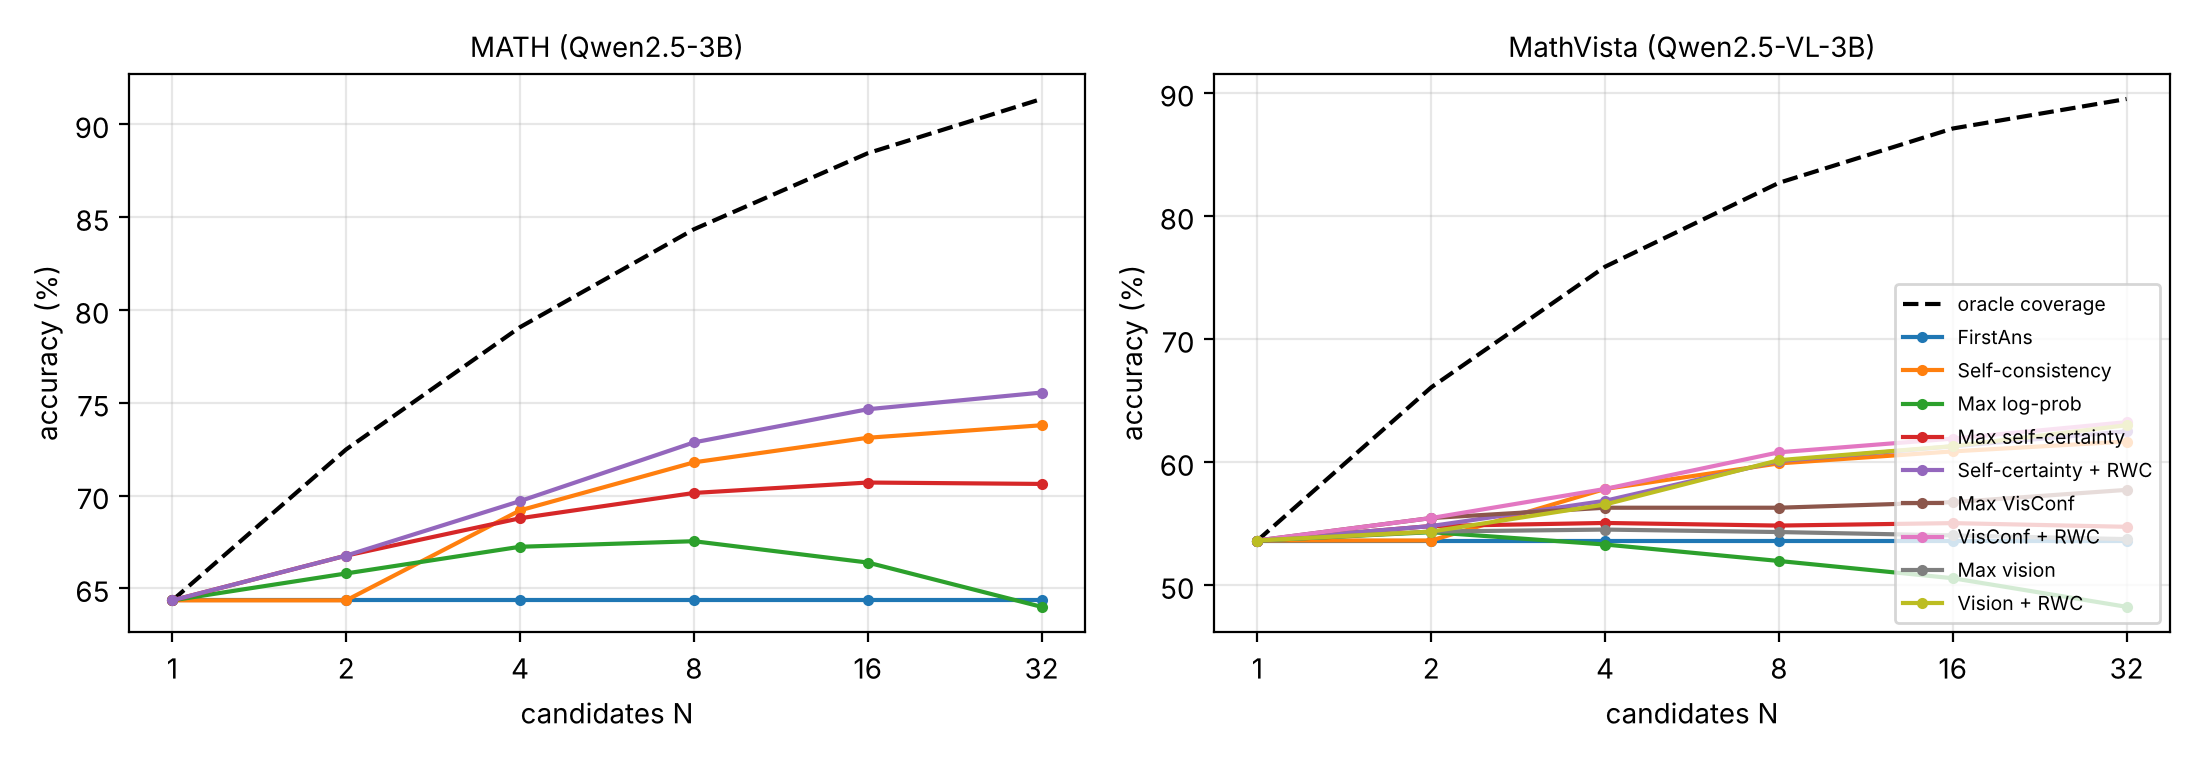
\includegraphics[width=\linewidth]{task3/report/scaling.png}
\caption{Accuracy and oracle coverage vs.\ number of candidates (held-out, averaged over 10 orders).}\label{fig:t3}
\end{figure}
\begin{table}[t]\centering\small
\begin{tabular}{lllrrrrl}
\toprule
dataset & method & required & acc@4 & acc@8 & acc@32 & tokens@32 & Δ vs SC @32 (pp) [95% CI] \\
\midrule
math & FirstAns & True & 64.3 & 64.3 & 64.3 & 669.8 & NaN \\
math & Max self-certainty & True & 68.8 & 70.1 & 70.6 & 21347.0 & -3.2 [-5.5, -0.8] \\
math & Max log-prob & True & 67.2 & 67.5 & 64.0 & 21347.0 & NaN \\
math & Self-certainty + RWC & True & 69.7 & 72.9 & 75.5 & 21347.0 & +1.8 [+0.7, +2.9] \\
math & Log-prob + RWC & False & 68.5 & 72.2 & 74.9 & 21347.0 & NaN \\
math & Self-consistency & True & 69.2 & 71.8 & 73.8 & 21347.0 & NaN \\
math & Shortest rollout & False & 65.2 & 64.6 & 62.4 & 21347.0 & -11.4 [-14.1, -9.0] \\
math & Oracle coverage & NaN & 79.1 & 84.3 & 91.4 & NaN & NaN \\
mathvista & FirstAns & True & 53.6 & 53.6 & 53.6 & 277.8 & NaN \\
mathvista & Max self-certainty & True & 55.1 & 54.9 & 54.8 & 8897.8 & -6.9 [-9.9, -3.7] \\
mathvista & Max log-prob & True & 53.3 & 52.0 & 48.2 & 8897.8 & NaN \\
mathvista & Max vision & True & 54.5 & 54.3 & 53.8 & 8897.8 & NaN \\
mathvista & Max VisConf & True & 56.3 & 56.3 & 57.8 & 8897.8 & NaN \\
mathvista & Max tokenwise fusion & False & 55.9 & 55.7 & 56.2 & 8897.8 & NaN \\
mathvista & Self-certainty + RWC & True & 56.9 & 60.1 & 62.5 & 8897.8 & +0.8 [-0.5, +2.2] \\
mathvista & Log-prob + RWC & False & 55.7 & 58.5 & 60.8 & 8897.8 & NaN \\
mathvista & Vision + RWC & True & 56.6 & 60.2 & 63.0 & 8897.8 & +1.3 [-0.2, +3.0] \\
mathvista & VisConf + RWC & True & 57.8 & 60.8 & 63.2 & 8897.8 & +1.6 [+0.2, +3.1] \\
mathvista & Tokenwise fusion + RWC & False & 57.6 & 60.9 & 62.7 & 8897.8 & NaN \\
mathvista & Self-consistency & True & 57.8 & 59.9 & 61.7 & 8897.8 & NaN \\
mathvista & Shortest rollout & False & 55.2 & 54.6 & 54.0 & 8897.8 & -7.7 [-10.7, -4.8] \\
mathvista & Oracle coverage & NaN & 75.9 & 82.7 & 89.5 & NaN & NaN \\
\bottomrule
\end{tabular}

\caption{Selection methods on held-out questions; $\Delta$ vs.\ self-consistency at $N=32$ with paired question-bootstrap CIs.}\label{tab:t3}
\end{table}
\todo{RQ1 coverage vs.\ selection (failure decomposition); RQ2 signals (quartile gaps, length control, c--v correlation, tokenwise fusion); RQ3 live strategies (accuracy, tokens, runtime, transitions); RQ4 adaptive stopping; RQ5 trade-offs and failures.}

\section{Conclusion}
\todo{One paragraph.}

\bibliographystyle{plainnat}
\bibliography{refs}

\appendix
\section{Implementation details and deviations}\label{app:details}

\subsection{Task 1}
\begin{table}[h]\centering\small
\begin{tabular}{lccccc}\toprule
 & Full FT & Full FT + L2-SP & LoRA-4 & LoRA-16 & OPLoRA-16 \\\midrule
Peak LR & $2\times10^{-5}$ & $2\times10^{-5}$ & $2\times10^{-4}$ & $2\times10^{-4}$ & $2\times10^{-4}$ \\
Rank $r$ / $\alpha$ & -- & -- & 4 / 8 & 16 / 32 & 16 / 32 \\
Protected directions $k$ & -- & -- & -- & -- & 128 \\
L2-SP $\lambda$ & 0 & $10^{-3}$ & -- & -- & -- \\
Trainable weights & FP32 & FP32 & FP32 adapters & FP32 adapters & FP32 adapters \\
Frozen weights & -- & -- & FP16 & FP16 & FP16 \\\bottomrule
\end{tabular}
\caption{Variant-specific settings. Shared: micro-batch 2 $\times$ 16 accumulation steps (effective batch 32), 1{,}250 updates, 38 warmup updates then cosine decay to 0, AdamW ($\beta=(0.9,0.999)$, $\epsilon=10^{-8}$, weight decay 0.01 on matrices only), gradient clipping 1.0, gradient checkpointing, FP16 autocast with dynamic loss scaling (initial scale 65{,}536). LoRA/OPLoRA adapt \texttt{q,k,v,o,gate,up,down\_proj} with dropout 0.05.}
\end{table}

\begin{itemize}
\item \textbf{Prompt format.} Each prompt is the chat template of the user turn with the non-thinking generation prefix (\texttt{<|im\_start|>assistant\textbackslash n<think>\textbackslash n\textbackslash n</think>\textbackslash n\textbackslash n}); the target is the response followed by \texttt{<|im\_end|>}. Only target tokens receive loss. This prefix is identical to the one used at evaluation and was checked against the template's rendering of a full conversation.
\item \textbf{Loss.} Summed token cross-entropy divided by the number of supervised tokens in the whole effective batch, so every token has equal weight regardless of how examples fall into micro-batches. The LM head is applied only at supervised positions.
\item \textbf{Schedule.} We use the Hugging Face cosine schedule with warmup, which starts at LR 0, so update 1 makes no parameter change.
\item \textbf{L2-SP.} The penalty $\frac{\lambda}{2}\|\theta-\theta_0\|^2$ covers all parameters. Its gradient $\lambda(\theta-\theta_0)$ is added after unscaling and before clipping, so clipping applies to the full objective. $\theta_0$ is an FP32 copy on the GPU, whose memory and time are reported as overhead. AdamW's decoupled weight decay (0.01) remains active in this run as in all others, so L2-SP acts on top of it.
\item \textbf{LoRA and OPLoRA.} Implemented from scratch (no PEFT). $A$ uses Kaiming-uniform initialization ($a=\sqrt5$, as in PEFT) and $B=0$; initialization is seeded per module name, so LoRA-16 and OPLoRA-16 begin from identical factors. OPLoRA computes the top-$k$ left and right singular vectors $U_k,V_k$ of each frozen $W_0$ once in FP32 and uses projected factors $\tilde B=(I-U_kU_k^\top)B$ and $\tilde A=A(I-V_kV_k^\top)$, so $\Delta W=\frac{\alpha}{r}\tilde B\tilde A$ is orthogonal to both subspaces. Projections run in FP32 outside autocast; the measured constraint residual is about $3\times10^{-7}$.
\item \textbf{Export check.} Adapters are merged into FP16 weights ($W_0+\Delta W$ computed in FP32) for evaluation. Merged and unmerged logits are compared, and the OPLoRA constraint is re-verified on the exported factors.
\item \textbf{Checkpoints.} Checkpoints are written at updates 312, 625, 937 and 1{,}250; weights at 625 and 1{,}250 are kept for evaluation. Only the newest checkpoint keeps optimizer state. Resuming from a checkpoint was verified to reproduce uninterrupted training exactly.
\item \textbf{Evaluation.} The primary metrics are flexible-extract exact match for GSM8K and \texttt{acc\_norm} for HellaSwag and ARC-Easy, \texttt{acc} for BoolQ. Because lm-eval does not pass \texttt{enable\_thinking} to the chat template, a small subclass renders it with thinking disabled, and the rendered GSM8K prompt is asserted to contain the empty think block. GSM8K uses the task's stock stop sequences and filters with a fixed generation batch of 64; likelihood tasks use no chat template.
\item \textbf{Diagnostics.} $\rho_k=\|U_kU_k^\top\Delta W\|_F^2/\|\Delta W\|_F^2$ (random baseline $k/d_{\text{out}}=0.125$); we also report the analogous input-side fraction. $R(z)=\|\Delta W z\|_2/\|W_0z\|_2$ uses the \texttt{down\_proj} input $z$ at the last prompt token, cached once from the starting model, so it isolates the local weight change and ignores changes in upstream layers. The 64 probes were sampled before any result was seen.
\item \textbf{Qualitative.} Each of the 24 prompts is answered greedily (512-token cap) by all seven conditions (168 responses). Automatic flags (JSON validity, template compliance, truncation, repeated 4-grams, math framing) support a manual annotation of 42 responses \todo{state the annotation rubric}.
\end{itemize}

\subsection{Task 2}
\begin{table}[h]\centering\small
\begin{tabular}{lccc}\toprule
 & Stage 1: captions & Stage 2: instruction & Stage 3: natural VQA \\\midrule
Updates & 2{,}250 & 1{,}500 & 750 \\
Connector LR & $10^{-3}$ & $10^{-4}$ & $5\times10^{-5}$ \\
LoRA LR & -- & $2\times10^{-5}$ & $10^{-5}$ \\
Mixture & cap.\ 1.0 & pres.\ .5, count.\ .25, cap.\ .25 & VQA .7, others .1 each \\\bottomrule
\end{tabular}
\caption{Stage settings (cap.\ = captions, pres./count.\ = generated presence/counting pairs). Shared: micro-batch 8 $\times$ 2 accumulation (effective batch 16), per-stage linear warmup over 5\% of updates then cosine decay to 10\% of peak, AdamW with weight decay 0.01 on matrices only, a fresh optimizer at each stage, clipping 1.0, FP16 autocast. LoRA: $r=16$, $\alpha=32$, dropout 0.05 on \texttt{q,k,v,o\_proj}.}
\end{table}

\begin{itemize}
\item \textbf{Visual features.} SigLIP's \texttt{last\_hidden\_state} was verified to equal the post-LayerNorm encoder output, so LayerNorm is applied exactly once. Images are resized to 224 (bicubic), rescaled by 1/255 and normalized with mean and std 0.5.
\item \textbf{Prompt.} \texttt{<|vision\_start|>}, 196 \texttt{<|image\_pad|>} tokens and \texttt{<|vision\_end|>} precede the text in the user turn; thinking is disabled. Captioning uses ``Write a short caption for this image.''; questions append the LLaVA-1.5 short-answer instruction~\cite{liu2023llava} ``Answer the question using a single word or phrase.''. For the no-image condition the whole vision block is removed and positions are recomputed. Prompts are identical across image conditions. Length caps: question 80, caption 64, answer 16 tokens.
\item \textbf{Loss.} Token-mean NLL within each example, averaged over examples in the effective batch.
\item \textbf{Data.} Captions: the first three captions (by annotation ID) of 6{,}000 train2014 images; 96 val2014 images form the caption dev set. Generated questions use COCO instances: a presence positive needs a non-crowd instance covering at least 0.5\% of the image, a negative has no annotation of the category, and counting images have 1--4 instances, all non-crowd and at least 0.5\% of the image. Training draws from pre-generated pools of 20{,}000 presence and 20{,}000 counting pairs over training images. VQAv2 pairs require at least 8 of 10 annotators to agree and both questions to share an answer type; the target is the most frequent original string in the consensus group. Development and test images come from val2014, and all five evaluation sets use mutually disjoint images (528 in total; 8{,}730 training images).
\item \textbf{Sampling.} Stage 1 makes two shuffled passes over the captions. In stages 2--3 each draw selects a component by its mixture weight and contributes a full question pair or two captions, so both members of a complementary pair are always in the same batch.
\item \textbf{Connector scale.} Fixed at initialization as the mean text-embedding norm divided by the mean connector-output norm on training data, and not trained \todo{value from \texttt{calibration.json}}.
\item \textbf{Evaluation.} Greedy decoding with a 16-token cap. VQA answers use the official normalization and soft accuracy, ported from the VQA evaluation script; normalization is also applied when all ten answers are identical. Mismatched images come from a fixed seeded derangement within each suite. The partner-follow rate scores each answer against the partner question's reference (exact match, or soft accuracy for VQA).
\end{itemize}

\subsection{Task 3}
\begin{itemize}
\item \textbf{Grouping and grading.} Equivalence is symmetric math-verify comparison without gold answers (cached, with timeouts). MathVista multiple-choice answers are mapped to option letters. All unparseable answers form one \textsc{no\_answer} group. Correctness is used only for evaluation and retrospective analysis, never for selection.
\item \textbf{Splits and orders.} Sorted question IDs are permuted with seed 6304; the first 200 form the development split and the rest the held-out split; the live run uses the first 50 held-out questions. Ten seeded rollout orders per question are shared by all methods. Results average over orders within a question, then over questions.
\item \textbf{Selection.} Score and vote ties go to the earliest supporting rollout in the current order. RWC weights the candidate ranked $r$ (average ranks for ties) by $(N-r)/(N-1)$ and sums weights within answer groups. VisConf's 5th and 95th KL percentiles are recomputed on each revealed candidate set with linear interpolation. Missing attention denominators are excluded from the visual score. A shortest-rollout selector serves as a length-only control.
\item \textbf{Cost.} Generated-token cost is the supplied retained token count \todo{confirm column against the data README}.
\item \textbf{Adaptive stopping.} After 4, 8 and 16 revealed rollouts, the agreement controller stops when a unique non-\textsc{no\_answer} leading answer has vote share $\ge\tau$, $\tau\in\{0.5,0.625,0.75,0.875,1\}$. The quality-aware controller also requires the RWC winner (self-certainty for MATH, VisConf for MathVista) to agree and its margin to be at least $\gamma\in\{0,0.1,0.25,0.5\}$. Otherwise it uses all 32. Both return the self-consistency answer at stopping. On the development split we choose the setting with the lowest mean cost whose accuracy is within 1\,pp of fixed-32 self-consistency (fixed-32 itself is always eligible), then freeze it.
\item \textbf{Live run.} Qwen2.5-3B-Instruct \todo{revision hash}, FP16, batch size 1, temperature 0.7, top-$p$ 0.8, top-$k$ 20, independently seeded calls, no gold feedback. The refinement prompt asks the model to review the shared first response, correct any errors and keep a correct answer. The revised answer is returned even when it has none (counted as \textsc{no\_answer}), with no fallback to the first answer.
\end{itemize}

\subsection{Reused code and tools}
The VQA normalization is ported from the official VQA evaluation script, MathVista answer normalization from the MathVista repository, and HellaSwag preprocessing from lm-evaluation-harness. The qualitative prompts are from the emergent-misalignment repository~\cite{betley2025emergent}. Code was written with help from an LLM coding assistant (Claude) and was reviewed and tested by the author.
\end{document}
